\chapter{Introduction to Robotics}
%------------------------------------------------

\section{What is Robotics?}
\par Robotics is an interdisciplinary field that integrates Computer Science and Engineering. It comprises design, construction, operation and use of robots. The field targets the creation of machines that can help and assist humans through blending aspects of mechanical engineering, electrical engineering, mechatronics, electronics etc
\paragraph{ } A Robot is an interactive machine capable of carrying out a complex series of actions automatically, especially one programmable by a computer, to reduce human risk in hazardous works. Thus, robotics is an interdisciplinary branch of engineering and science that deals with the design, construction, operation, and use of robots, as well as computer systems for their control, sensory feedback, and information processing to create an efficient robot. A robot can be thought as an combination of sensors, controllers and actuators. Sensor provide collection of information from environment, that are processed by controllers who generate signal to actuators to interact with environment.
\paragraph{ } Robots are put to use in different applications. Their usage is determined by the field they concentrate on. Robotics is a vast field. They may be manufactured or processed in different forms, shapes and utility. Joseph Engelberger, godfather of robotics, once said \textit{“I can't define a robot, but I know one when I see one.”}

\section{Evolution of Robotics}
\par The question of evolution of robotics take us to the ancient world and era of industrial revolution. Engineers were trying to develop machines that can handle dangerous tasks for automotive industry and defence. Robots they developed were meant to be a replica of human actions.

\newpage
\begin{fullwidth}
    \centering
    \textbf{\textit{Major Events in the Evolution of Robotics}}
     \begin{figure*}[h!]
        \centering
        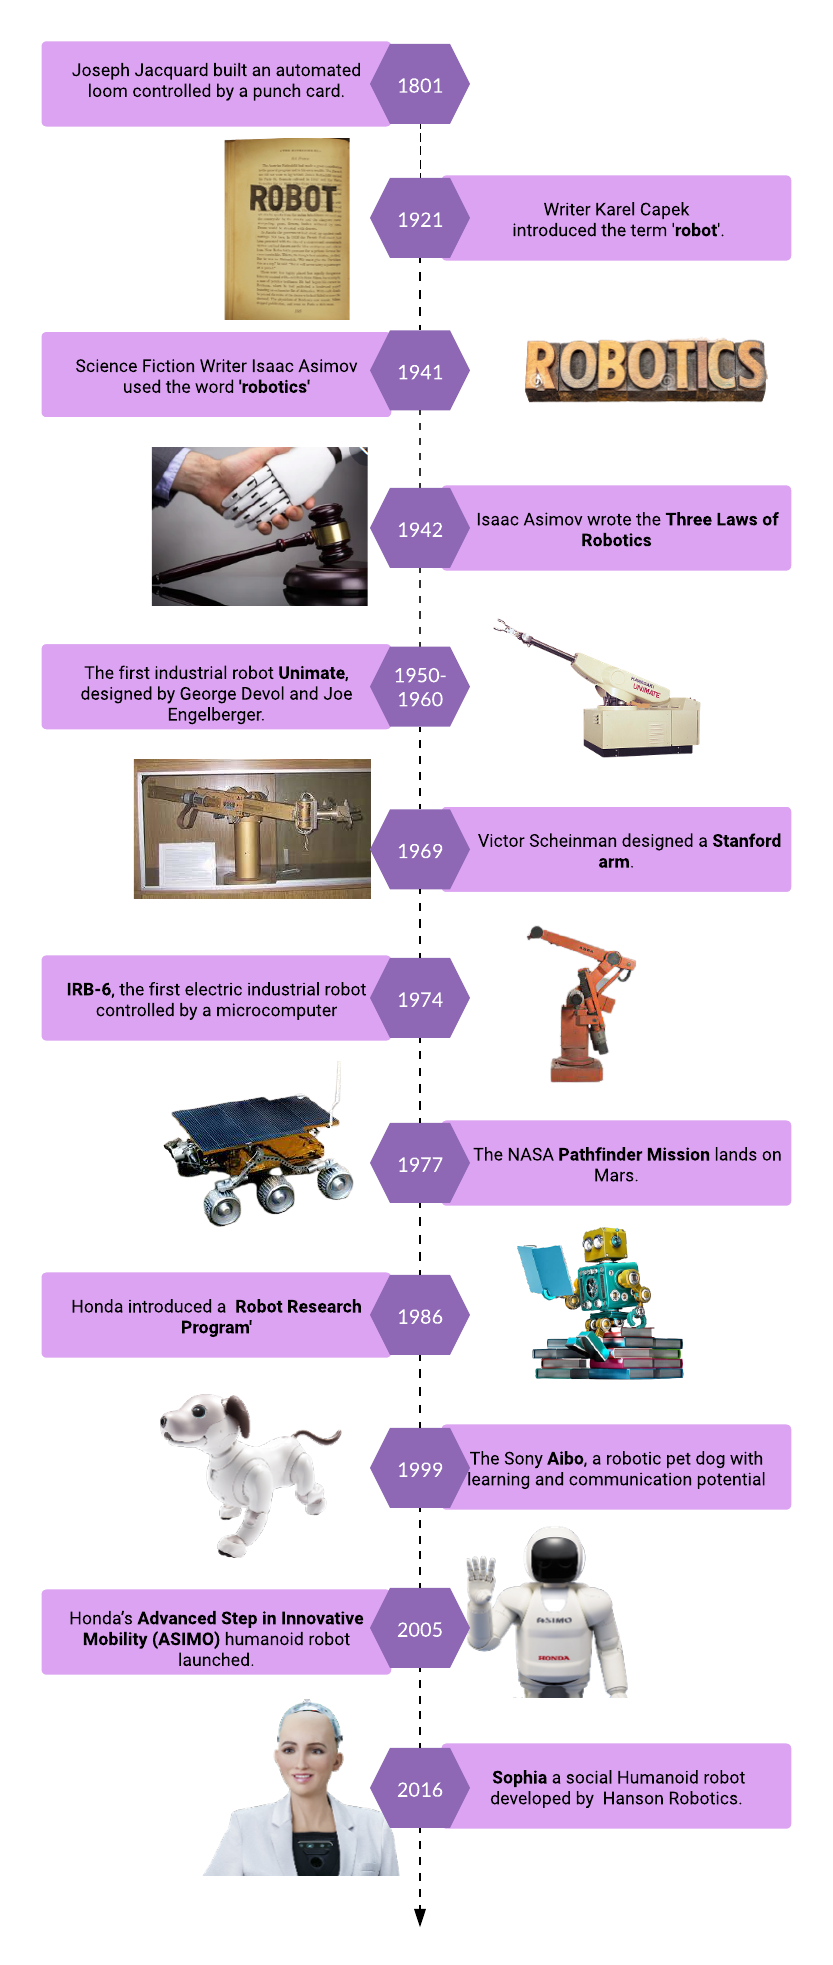
\includegraphics[height=8.1in]{Images/Intro_robotics/Timeline.png}
    \end{figure*}
\end{fullwidth}

\paragraph{ } Further advancements in the technical sphere since the 2000's have led to more advanced automation and innovation. The improvements in the fields of Machine Learning and \ac{AI} again paves great milestones in the evolution of robotics. Automated machines have turned to be common comrades in industries like manufacturing, maritime explorations, military, agri-technologies. \ac{AI} is utilized to assess environments and act according to the programmed goals. Recent developments have also led to the use of these technologies in data and predictive analytics to provide user friendly recommendations to improve the customer satisfaction. The developments in this realm is certainly going to rule the pulse of the impending technical world.

\section{The Future of Robotics}
\par 